% Section 3: the replication (E5, H1). Sources: FINDINGS s19-s21, s25; CLAIMS A1-A6, A9, A10, F2, G8.
% One sentence per line; each result sentence names its FINDINGS section (s##) and CLAIMS row in its trailing comment.
\section{Replication}
\label{sec:replication}

\subsection{Hypothesis and test}

The replication (E5) asked whether, inside C3DGS and at equal rate over the three colour thresholds, OGC's Gram-metric VQ beats C3DGS's own colour VQ (P1, BD-PSNR of \code{ogc\_gram} against \code{c3dgs}) and beats the same Lloyd with the metric's trace (P2, \code{ogc\_gram} against \code{ogc\_scalar}), on the seven gate scenes. % Am17 d
It runs OGC's released VQ code (\code{gram\_kmeans}, unedited) on this project's estimate of OGC's metric (Section~\ref{sec:setup}), not on OGC's own Gram computation. % Am17 b; s16; E4
Both primaries were tested with the three criteria of Section~\ref{sec:setup}, before fine-tuning, on four processes per scene. % Am17 d; s19

\subsection{Result (pre-registered)}

E5 passed as pre-registered: both primaries met all three criteria with $n = 7$, no scene dropped, no primary row or value missing, and no process deferred, cut, rerun or stopped. % s19 "The verdict"; A1
OGC's VQ led C3DGS's own on every scene, with $\bar P_1 = 0.3558$ dB against $2\,\mathrm{SE}_{\mathrm{noise}} = 0.0065$ dB, from 0.1486 dB on truck to 0.4841 dB on bonsai (Table~\ref{tab:t1}). % s19 per-scene table; A2
The Gram metric led its trace on every scene, with $\bar P_2 = 0.1874$ dB against $2\,\mathrm{SE}_{\mathrm{noise}} = 0.0003$ dB. % s19 per-scene table; B1
Every one of the 14 per-scene values lay more than $2\,\mathrm{SE}_{\mathrm{noise}}$ above zero. % s19 "The verdict"; A1

\begin{table}[t]
\centering
\small
\caption{E5's primaries per scene (dB), as the verdict compared them (9 decimals). $D_s$ is the mean of the two $j = 0$ processes' paired difference. Pre-registered; generated from the committed bundles.}
\label{tab:t1}
% FINDINGS section 19, The verdict (E5, kaggle/gn_e5/S1-S3/gn5/)
% generated by paper/figs/t1_e5_primaries.py from committed bundles; do not edit
\begin{tabular}{lrrrr}
\toprule
Scene & P1 (dB) & P1 pair, $D_s$ & P2 (dB) & P2 pair, $D_s$ \\
\midrule
bonsai & 0.484060073 & 0.662099426 & 0.320522033 & 0.418902629 \\
counter & 0.319226727 & 0.449111462 & 0.165453427 & 0.205868244 \\
kitchen & 0.411145219 & 0.631160777 & 0.275679656 & 0.378012426 \\
room & 0.386923539 & 0.540365366 & 0.175005021 & 0.218052008 \\
truck & 0.148587944 & 0.248380899 & 0.100030562 & 0.149408519 \\
drjohnson & 0.276526313 & 0.446854649 & 0.128071281 & 0.170944156 \\
playroom & 0.464370802 & 0.689506991 & 0.147096105 & 0.180252437 \\
\midrule
$\bar P$ ($n = 7$) & 0.355834374 &  & 0.187408298 &  \\
SD\_pool & 0.012122221 &  & 0.000627531 &  \\
SE\_noise = SD\_pool / $\sqrt{14}$ & 0.003239800 &  & 0.000167715 &  \\
2 $\times$ SE\_noise & 0.006479600 &  & 0.000335429 &  \\
scenes with P > 0 & 7 (5 needed) &  & 7 (5 needed) &  \\
\bottomrule
\end{tabular}

\end{table}

Across the seven scenes P1 had a standard deviation of 0.1175 dB ($t = 8.01$) and P2 one of 0.0805 dB ($t = 6.16$); these scene-level statistics were not pre-registered. % s19 "Exploratory"; A3
Under the standard error that matches one curve per scene, $\mathrm{SD}_{\mathrm{pool}}/\sqrt{n}$, P1 lay 77.66 and P2 790.14 standard errors above zero, so criterion 3 held under either convention (analysis only). % s25; A1, A2, B1

\subsection{A fresh run (descriptive)}

The fine-tuning experiment (E6 part (b)) recomputed P1 in new processes on the same scenes, as a report-only secondary. % s21 secondary 1; F2
It read $\bar P_1 = 0.3556$ dB against E5's 0.3558 dB, positive on 7 of 7 scenes, each scene within 0.0045 dB of E5's value. % s21 secondary 1; F2
Seeded C3DGS runs are not reproduced bit for bit on the GPU, so the two runs differ in geometry; the agreement is between runs, not a repeat of the same arithmetic. % s15; s22 f; E2, F2

\subsection{Implementation check (descriptive)}

The derived reimplementation \code{ogc\_gram\_ours} reproduced OGC's labels, float codebook and \code{.npz} bytes exactly in every process: 28 in E5 and 4 in the pilot on train. % s19 secondaries; s18; A6
It also equalled OGC's row in all 12 processes of the development scenes. % s23 "Mechanics notes"; G8

\subsection{Robustness to the evaluation (exploratory)}

Under C3DGS's own evaluation, \code{ogc\_gram} minus \code{c3dgs} at $j = 0$ averaged $+0.5205$ dB against $+0.5239$ dB under protocol~ii, positive on every scene under both. % s20 "C3DGS's own evaluation"; A9
This comparison is at $j = 0$ only, so it is not a BD value. % s20; A9
SSIM and LPIPS agreed with PSNR in sign on every scene, at $j = 0$ and in BD, for both primary pairs: P1's pair had a mean BD-SSIM of $+0.0071$ and BD-LPIPS of $-0.0089$, and P2's pair $+0.0036$ and $-0.0052$. % s20 "SSIM and LPIPS"; A10
The BD on SSIM and LPIPS reuses E5's fit with those metrics in place of PSNR and was not pre-registered. % s20; A10

\subsection{The curves}

Figure~\ref{fig:f1} shows each scene's two curves before fine-tuning (left panels) from E6 part (b)'s processes, the same processes whose fine-tuned rows appear in the right panels; E5's P1 of record comes from E5's own processes. % Fig.1 caption source: paper/figs/f1_rd_curves.py; s21 secondary 1

\begin{figure}[t]
\centering
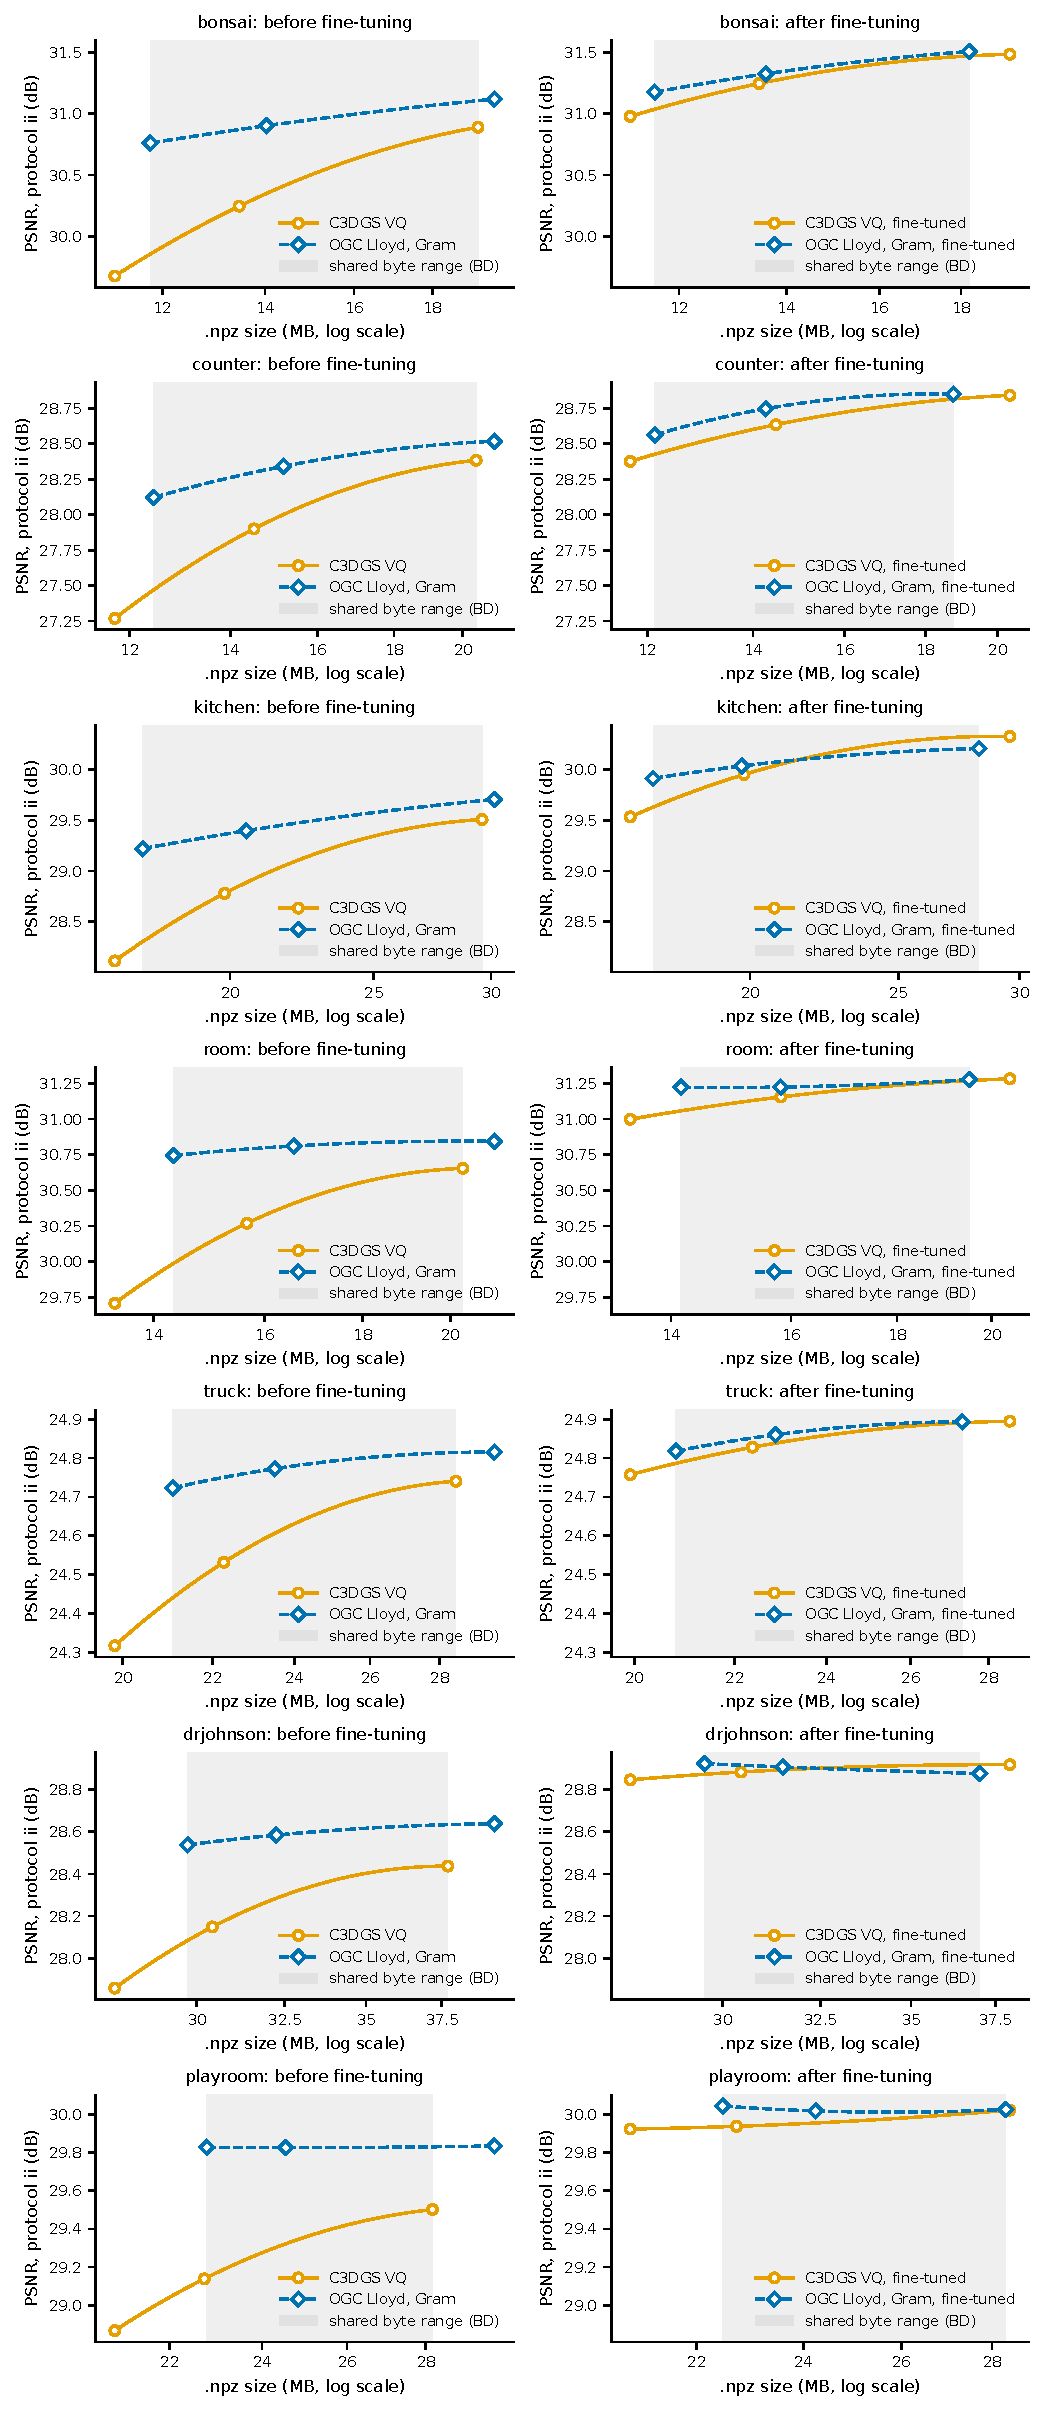
\includegraphics[width=\linewidth]{f1_rd_all.pdf}
\caption{Protocol~ii PSNR against \code{.npz} size (log scale) per gate scene, before (left) and after (right) C3DGS's fine-tuning, from E6 part (b): one process (seed 0) per point, each curve the parabola through its three points. The shaded band is the byte range the two curves share, over which BD-PSNR averages. The two panels of a scene share the PSNR axis.}
\label{fig:f1}
\end{figure}

\subsection{Caveats}

The test runs OGC's released VQ on this project's 16-probe estimate of OGC's metric, not on OGC's own Gram computation, so this replication (H1) replicates OGC's VQ given an estimated metric; a difference between our $G$ and OGC's own Gram, such as the trace shortfall on train (Section~\ref{sec:setup}), lies outside this test. % Am17 b; s16; E4
The result covers seven scenes, INRIA's published checkpoints, $K$~=~4,096 and three colour thresholds, on one host commit, one GPU type and one software image. % s19 "What E5 settles"; CLAIMS common E5 limits
Five of the seven scenes had been used earlier by this project with its own checkpoints, and four appear in OGC's paper (Section~\ref{sec:setup}). % Am15 d; CLAIMS common E5 limits
$\mathrm{SE}_{\mathrm{noise}}$ is seed noise at $j = 0$ only; it does not include how P varies from scene to scene, and the points at $j = -1$ and $j = +1$ have one seed each, so the noise of the BD values themselves was not measured. % s19 "What E5 settles"; A2; CLAIMS Gap 8
Each P rests on six measurements, since a parabola through three points per curve fits them exactly. % s19; A2
Before fine-tuning, the $j = 0$ difference of $+0.5239$ dB (95\% interval $+0.3798$ to $+0.6681$) sits beside OGC's reported $+0.49$ dB, but the two are not like for like: OGC's is a paired mean over nine Mip-NeRF 360 scenes, one run each, under its own evaluation and at a larger size than its reproduction, ours over seven scenes, four of them shared, under protocol~ii and at unequal bytes. % s19 secondaries; A4; RELATED_WORK_OGC.md section 2 g (OGC's Table 1)
